\def\bbeta{\boldsymbol{\beta}}

% declaration of the new block
\algblock{ParFor}{EndParFor}
% customising the new block
\algnewcommand\algorithmicparfor{\textbf{parallel for}}
\algnewcommand\algorithmicpardo{\textbf{do}}
\algnewcommand\algorithmicendparfor{\textbf{end\ pararell for}}
\algrenewtext{ParFor}[1]{\algorithmicparfor\ #1\ \algorithmicpardo}
\algrenewtext{EndParFor}{\algorithmicendparfor}

\chapter{\;\;Predicting task activation maps from task-free resting-state data}\label{chap:rsfmri2tfmri}
\markright{{~{\rm \ref{chap:rsfmri2tfmri}}. Predicting task activation maps from task-free resting-state data}\hfill}{}

\minitoc

\section{Introduction}
Across-subject variability in organization is a hallmark of the human
brain, that reflects genetic variability and is in turn reflected in
behavioral differences.
%
It has resisted so far modeling attempts, leading to blurred
population-level anatomical templates and high-variance in
functional representations across individuals.
%
The only solution to defeat this variability is actually to condition
individual representations on other data, for instance, mapping
functional organization subject to anatomical constraints, or relevant
features of brain organization, such as structural or functional
connectivity \citep{saygin2011}.

  In neuroimaging and cognitive neuroscience, it is widely believed that the functional
  connectivity (FC)
  structure at rest remains grossly unchanged during task-stimulus presentation. This makes sense
  by
  least-action principle considerations:
  the brain does not need to rewire the functional links between regions upon presentation of a
  stimulus:
  it conserves the same networks as during rest, except that some edges are strengthened while
  others
  are weakened, to support the cognitive load of the particular task. Pushing this even further,
  one can claim that the resting-state FC of the brain predictively modulates the functional
  responses
  of the brain in the presence of task. Indeed, recently, resting-state fMRI has been shown to provide relevant
constraints for functional mapping, opening the possibility to capture
in standardized and cheaper acquisition most of the inter-individual
differences \citep{tavor2016task,cole2016,bzdok2016}.
%
Possible applications include the improvement of population-level
analyses, e.g. by finding better imputation schemes when dealing with
missing data, detecting outlier data, and clarifying between-subjects
similarities in comparison with genotyping or behavioral data.
%
An important practical question has become how to optimize information
transfer across these modalities to boost the chance of capturing the
essence of inter-individual differences.

\paragraph*{\textbf{Our main contributions.}}
In this work, we propose a general framework for the problem of predicting task fMRI activation maps from resting-state-only features.
We present 2 main contributions: \textit{(a)} the stacking of data across different
random subsets subjects to reduce model-complexity and improve the prediction on held-out subjects, and
\textit{(b)} a multi-target regression approach to the
predictive problem which better captures the functional inter-dependencies between different cognitive tasks.
% \textit{(c)} bagging of predictions across different random
% parcellations to reduce variance.
%
This generalizes and improves on the ideas in \citep{tavor2016task}.
We demonstrate the empirical gains brought by this approach through
experiments on real datasets.

\section{Feature extraction}
\label{sec:fe}
The goal is to extract from resting-state data, pertinent features
that encode the functional connectivity information in each voxel.
%
A na\"ive choice would be to use the adjacency vector of each
voxel in the whole-brain functional connectivity matrix. 
%
This is not practical due to the large number of (noisy) voxels, as it
leads to enormous feature matrices. However, due to the inherent local
correlations of data from different voxels,
%
all this information is captured in the affinity of each voxel to a set
of brain regions or networks.
%
One way to get such profiles is to automatically learn a
low-dimensional reduction of the resting-state data $\B{X}_s \in \mathbb R^{n_s \times p}$ of
each subject $s$ into a
common latent space, of dimension $k \ll \min(\min_s(n_s), p)$, as
proposed in \citep{tavor2016task}. Here, $n_s$ is the number of TRs (Repetition Time)
and $p$ is the number of voxels.

\begin{marginfigure}%[!htbp]
  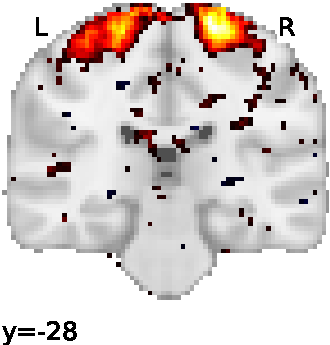
\includegraphics[width=.47\linewidth]{figures/global_dict.pdf}  
  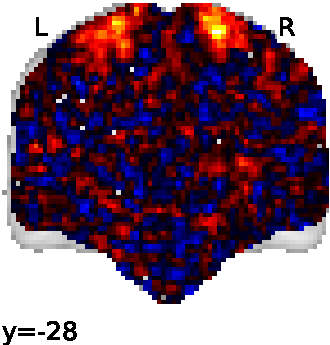
\includegraphics[width=.47\linewidth]{figures/subject_dict.pdf}
  \caption{FC feature-extraction. \textbf{Left:} A component of the
    group dictionary.  \textbf{Right:} Corresponding component for
    an individual subject's dictionary estimated using the proposed formula
    \eqref{eq:mr}.}
  \label{fig:fe}
\end{marginfigure}

\subsection{Dual regression}
As before, let the $n_s$-by-$p$ matrix $\B{X}_s$ be the resting-state data for subject $s$ and
$\B{D}$ be the $k$-by-$p$ group-level dictionary (aka \textit{topographic basis}) obtained by
stacking together resting-state
time-series data from all the subjects and decomposing into $k$ components of $p$ voxels each by
running a multi-subject decomposition algorithm like PCA, ICA, or dictionary-learning, etc.
(more details on obtaining $\B{D}$ later).
%
We assume $\B{D}$ to be under-complete -- i.e $k \ll \min(\min_s(n_s), p)$--
and therefore full-rank (i.e $\B{D}\B{D}^T$ is invertible).

The standard
``dual-regression'' procedure\citep{tavor2016task} then proceeds as follows:
\begin{itemize}
\item Compute the $n_s$-by-$k$ matrix of subject-to-components temporal dynamics $\B{C}_s$
  by regressing the group-level dictionary $\B{D}$ onto subject data $\B{X}_s$:
  \begin{equation}
  % \B{X}_s \approx \B{C}_s\B{D}.
    {\B{C}}_s \in \text{argmin}_\B{C} \|\B{X}_s - \B{C}\B{D}\|^2_{\text{Fro}}
    \label{eq:dr1}  
    \end{equation}
% \textbf{XXX rather write it: }
  \item Compute individual dictionary $\tilde{\B{X}}_s$ by regressing subject-to-components temporal
    dynamics $\B{C}_s$ onto subject data $\B{X}_s$:
  \begin{equation}
    % \B{X}_s \approx \B{C}_s\tilde{\B{X}}_s.
    \tilde{\B{X}}_s \in \text{argmin}_\B{Z} \|\B{X}_s - \B{C}_s\B{Z}\|^2_{\text{Fro}}
    \label{eq:dr2}
  \end{equation}%\textbf{XXX idem}
\end{itemize}
The end result is that for each subject $s$ and each voxel $v$, we
obtain $k$ scalars,  namely the $vth$
column of $\tilde{\B{X}}_s$, which represent the functional-connectivity profile w.r.t the group-level $k$-dimensional latent space.
These are the features (see Fig. \ref{fig:fe}).

\subsection{Using only a single regression step}
For the standard ``dual-regression'' feature-extraction method\citep{tavor2016task},
a total of 2 regression steps are done (hence the name of the procedure).
As a first (conceptual) improvement, we note that the individual dictionary
$\tilde{\B{X}}_s = \B{C}_s^\dagger\B{X}_s$ can be rewritten as
\[
  \begin{split}
    \tilde{\B{X}}_s  &= (\B{C}_s^T\B{C}_s)^{-1}\B{C}_s^T\B{X}_s
    \\
    &= ((\B{D}\B{D}^T)^{-1}\B{D}\B{X}_s^T\B{X}_s\B{D}^T(\B{D}\B{D}^T)^{-1})^{-1}(\B{D}\B{D}^T)^{-1}\B{D}\B{X}_s^T\B{X}_s\\
    &= \B{D}\B{D}^T(\B{D}\B{X}_s^T\B{X}_s\B{D}^T)^{-1}\B{D}\B{X}_s^T\B{X}_s\\
    &=
    \B{D}\B{D}^T\underbrace{\B{D}\B{X}_s^T(\B{X}_s\B{D}^T\B{D}\B{X}_s^T)^{\dagger}\B{X}_s}_{\text{OLS}(\B{X}_s\B{D}^T,\B{X}_s)}.
    \end{split}
  \label{eq:mr}
\]
That is, we regress the $n_s$-by-$k$ matrix $\tilde{\B{C}}_s := \B{X}_s\B{D}^T$
  onto the subject's resting-state time-series data $\B{X}_s$ and then
  reweight the result by the component-to-component covariance matrix $\B{D}\B{D}^T$ of the group-level dictionary. All in all, only a 1 regression step
  is needed.

\subsection{Obtaining the global dictionary $\B{D}$}
Since the resting-state time-series data are large (for example $1200$ 3D volumes of
$2 \times 10^5$ voxels in each subject in the HCP --Human Connectome Project-- dataset \citep{VanEssen20122222}), a decomposition
method that scales well is required. We use a variant of online
dictionary-learning method \citep{mairal2010}, a very fast
implementation of which has been proposed in
\citep{mensch2016dictionary}, based on random \textit{matrix sketching
  / sub-sampling}.
Incremental PCA/ICA-base methods\citep{smith2014group,varoquaux2010group} are also a competitive choice.
% Group-PCA \citep{smith2014group} is also a competitive choice.
% as was done in \citep{tavor2016task}.
% \begin{itemize}
%   \item Each subject is thus treated as an
%     observation of the statistics of the population.
%     \item Given
% this assumption, we will demonstrate that the unmixing
% matrix produced from the group ICA analysis will
% be largely separable across subjects.
% \end{itemize}

% \begin{itemize}
% \item Genesis: resting-state fMRI (rsfMRI) predicts task \citep{thirion2014principal,tavor2016task}; multi-subject
%   dict-learning (batch-mode) \citep{varoquaux2011multi,abraham2013}
% \item Saad Jbabdi says ``To scale to big data (think of concatenated 500+ subjects of rs HCP data),
%   Tavor et al. used MIGP (MELODIC's Incremental Group-PCA) \citep{smith2014group}''
% \item He [Tavor] also says ``Removing all the structural features (mylenation), etc.''
%   the model performs almost as before.
% \item Can / should use fast online dictionary learning algorithms like Mairal 2010.
% \end{itemize}

% \textbf{XXX Overall this section seems too long given that this is nort your main point. Will have to be shortened or removed (keep it for journal version ?)}

\subsection{Relationship between dual-regression and hyper-alignment}
\label{sec:haIsDr}
It turns out that the ``hyper-alignment'' (HA) framework \citep{haxby2011} and the ``dual regression'' (DR) scheme
\citep{tavor2016task} we just presented are very closely related.
% more or less the same technology.
Indeed,  \citep{haxby2011} considers the following problem

\begin{eqnarray}
  \begin{split}
    &\text{minimize }\frac{1}{2N}\sum_{s=1}^N\|\B{X}_s - \A\tilde{\B{X}}_s\|^2_{\text{Fro}}\\
    &\text{ over }
  \A \in \mathbb R^{n \times k},\;\tilde{\B{X}}_1,\ldots,\tilde{\B{X}}_N \in \mathbb R^{k \times p},
  \\
  &\text{ subject to }\tilde{\B{X}}_s\tilde{\B{X}}_s^T = \Id_k,\; \forall s \in [1\ldots N].
  \end{split}
\end{eqnarray}
This can be solved via a simple EM (\textit{expectation maximization}) algorithm:

\begin{itemize}
\item \textbf{M-step:} $\tilde{\B{X}}_s^{(k)} = \U_s^{(k)}{\V_s^{(k)}}^T\; \forall s$, where ${\A^{(k)}}^T\B{X}_s = \U_s^{(k)}\boldsymbol{\Sigma}_s{\V_s^{(k)}}^T$ is an SVD
\item \textbf{E-step:} $\A_s^{(k+1)} = \frac{1}{N}\sum_{s=1}^N\A_s^{(k)}$, where $\A_s^{(k)} := \B{X}_s{{}\tilde{\B{X}}_s^{(k)}}^T$
\end{itemize}

However DR is much more attractive due to its low cost: HA performs an SVD per subject per iteration.

\section{Bags of low-rank multi-target linear models}
\label{sec:bags}
% \paragraph*{\textbf{Why bootstrap sub-samples of more than 1 subject each?}}
Training on bootstraps of sub-samples of subjects instead of on a subject-by-subject
basis enforces a reduction in the complexity of the model without loss in capacity.
The idea is that the regression coefficients from predicting task activations
from resting state should be partly shared across subjects. 
%
This reflects the hypothesis that the global cognitive organization of the brain should share some
similarities across different subjects.

\begin{marginfigure}
  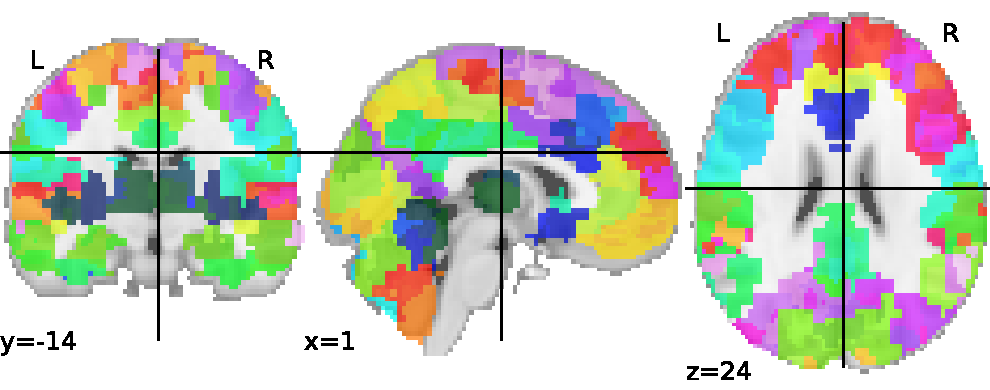
\includegraphics[width=1\linewidth]{figures/parcellation_00.pdf}
  \caption{A \textbf{parcellation} is simply a collection of contiguous /
    simply-connected masks $\mathcal P$ called \textbf{parcels} (the colored patches)
    which cover the brain. Each \textbf{voxel} of the brain belongs / is assigned to exactly one
    parcel. In the parcellation shown here, each parcel contains approximately 1000 voxels.}
  \label{fig:parcels}
\end{marginfigure}

Thus, for a bootstrap sub-sample $\mathcal S$ of $b$ ($1 \le b \le N$)
subjects, let $\tilde{\B{X}}_{\mathcal S} = [\tilde{\B{X}}_1|\ldots|\tilde{\B{X}}_b] \in
\mathbb R^{k \times p'b}$ be functional features masked over a parcel $\mathcal
P$ of $p' \le p$ voxels (see Fig. \ref{fig:parcels}) and horizontally stacked
matrix of functional features. Similarly, let $\B{Y}_{\mathcal S} \in \mathbb
R^{p'b \times c}$ be corresponding activation maps to the $c$ task contrasts,
masked over the same parcel, and stacked vertically. The goal is to link these
functional features with activations maps corresponding to $c$ task-activation
contrasts e.g. "Story-vs-Math", "Faces-vs-Houses", ``2Back-vs-0Back'', etc.

 Because there
might be strong cognitive inter-dependencies in these contrasts, it is reasonable to assume
that some of the coefficients in such a regression model will be shared across different
contrasts. 

\subsection{Low-rank Ridge regression}
\label{sec:lrrr}
Intra-subject activation maps for so-called different experimental stimuli may be
correlated to one another. Indeed one would expect all brain activations to any conceivable
experiment to be driven by a restricted set of latent causes, which is much less than
the number of possible experiments. Thus in an experiment with a sufficiently large
bail of experimental conditions, one would expect that corresponding
action maps would be correlated across different experimental conditions. Fitting a separate
model per experimental condition would therefore be statistically inefficient due to
model over-specification. We need a principled way to incorporate the covariance structure
of the intra-subject activation maps into our predictive model.
% \begin{figure}
%   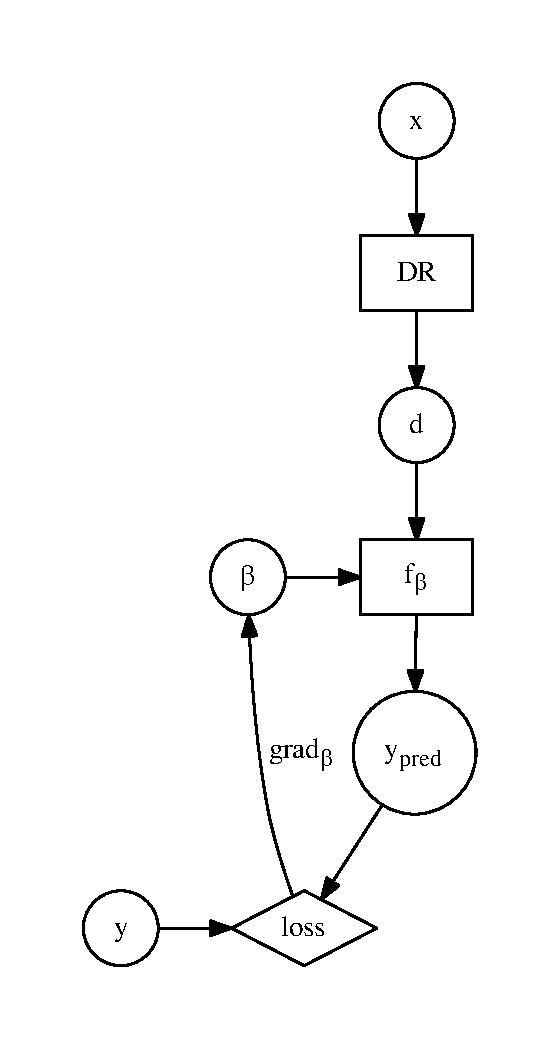
\includegraphics[width=1\linewidth]{figures/rfmri2tfmri.pdf}
%   \caption{\textbf{Training for 1 subject.} Dual-regression (DR) is applied to an incoming image patch $\B{x}$ to produce spatial features $\B{d}$ ($k$ features per-voxel). This is fed into a parametrized model which attempts to predict the task-activation this patch, over all the different contrasts jointly. The predicted activation is compared with true, and the prediction error is back-propagated to update the model parameters. Note that in case the prediction model is linear / affine (e.g as in Ridge regression), this learning can be done in closed form.}
% \end{figure}
Low-rank linear models do just this. It provides a with a smaller and tighter model (in
terms of number of free parameters) which best explains the covariance structure
between activation maps $\B{Y}$ for the different conditions. This can be written as
\begin{eqnarray}
  \begin{split}
    &\text{ Find }\bbeta_{\mathcal S} \in \mathbb R^{k \times c},
    \text{ with rank}(\bbeta_{\mathcal S}) \le r,\\
    &\text{ s.t }\B{Y}_{\mathcal S}^j
    \approx \tilde{\B{X}}^T_{\mathcal S}\bbeta_{\mathcal S}^j\; \forall j \in [1 \ldots
    c],
  \end{split}
      \label{eq:lrank}
\end{eqnarray}
for a chosen rank bound $r$, with $1 \le r \le \min(c, k)$.  The
model \eqref{eq:lrank} can be captured by the following convex program
\begin{equation}
  \begin{split}
    &\text{minimize } \frac{1}{2}\|\B{Y}_{\mathcal S} -
    \tilde{\B{X}}^T_{\mathcal S}\bbeta_{\mathcal S}\|_{\text{Fro}}^2 \text{ w.r.t
    }\bbeta_{\mathcal S} \in \mathbb R^{k\times c}\\
    &\text{ subject to rank}(\bbeta_{\mathcal S}) \le r.
  \end{split}
  \label{eq:lrrr}
\end{equation}
  This defines a low-complexity linear model
\begin{eqnarray} \hat{f}_{\mathcal S} : \tilde{\B{X}}_s \mapsto
\tilde{\B{X}}_s^T\hat{\bbeta}_{\mathcal S}
  \label{eq:lrrr_f}
\end{eqnarray} for predictively linking resting-state data to individual
activation maps over the parcel $\mathcal P$.  The full-rank case $r = \min(c,
k)$ together with the choice $b=1$ (no bagging) corresponds to the subject-wise
contrast-wise single-output linear regression model proposed in
\citep{tavor2016task}.

Now, let $\hat{\B{Y}}_{\mathcal S}^{\text{OLS}} = \U \boldsymbol{\Sigma} \V^T$ be the SVD
(singular-value decomposition) of the least-squares prediction
$\hat{\B{Y}}_{\mathcal S}^{\text{OLS}} := \tilde{\B{X}}_{\mathcal S}\hat{\bbeta}_{\mathcal S}^{\text{OLS}}$ where
$\hat{\bbeta}_{\mathcal S}^{\text{OLS}} := (\tilde{\B{X}}_{\mathcal S}^T\tilde{\B{X}}_{\mathcal S})^\dagger\tilde{\B{X}}_{\mathcal S}^T\B{Y}_{\mathcal S}$
is the ordinary least-squares (OLS) solution to the unconstrained version of \eqref{eq:lrrr}.
Of course \eqref{eq:lrrr} may fail to have a unique solution. The following elementary lemma,
whose proof  (Supp. Mat.) follows directly from the \textit{Eckart-Young-Mirsky theorem}~\citep{eckart2000}
and the orthogonality property of the OLS fit, produces a solution for model \eqref{eq:lrrr}. Viz,
\begin{lemma}
   A solution to \eqref{eq:lrrr} is given by
$\hat{\bbeta}_{\mathcal S} = \hat{\bbeta}_{\mathcal S}^{\text{OLS}}\boldsymbol{\Pi}_{\mathcal S}(r)$
  where $\boldsymbol{\Pi}_{\mathcal S}(r) = \sum_{i=1}^{r}\v_i\v_i^T$ is the orthogonal
  projector onto the subspace spanned by the first $r$ principal singular vectors $\v_{i \le r}$
  of the OLS prediction $\hat{\B{Y}}_{\mathcal S}^{\text{OLS}}$.
  \label{thm:eym}
\end{lemma}

It should be noted that the form of the solutions provided by the above lemma is particularly
  appealing: We only need to do a single fit to obtain a solution to problem \eqref{eq:lrrr}
  from solutions to the unconstrained OLS version of \citep{tavor2016task}.


\begin{proof}
Indeed, by the orthogonality property of least-squares estimates, we have the
  decomposition
 $$\|\B{Y}_{\mathcal S} - \tilde{\B{X}}_{\mathcal S}\bbeta_{\mathcal S}\|_{\text{Fro}}^2 = \|\B{Y}_{\mathcal S} - \hat{\B{Y}}_{\mathcal S}^{\text{OLS}}\|_{\text{Fro}}^2
 + \|\hat{\B{Y}}_{\mathcal S}^{\text{OLS}} - \tilde{\B{X}}_{\mathcal S}\bbeta_{\mathcal S}\|_{\text{Fro}}^2,$$
 with the first summand being independent of the model parameters $\bbeta_{\mathcal S}$.
Thus \eqref{eq:lrrr} can be rewritten as

\begin{equation}
  \begin{split}
    &\text{minimize } \frac{1}{2}\|\hat{\B{Y}}_{\mathcal S}^{\text{OLS}} - \tilde{\B{X}}_{\mathcal S}\bbeta_{\mathcal S}\|_{\text{Fro}}^2\text{ w.r.t }\bbeta_{\mathcal S} \in
    \mathbb R^{k\times c}\\
    &\text{ subject to rank}(\bbeta_{\mathcal S}) \le r.
    \end{split}
  \label{eq:lrrr_bis}
\end{equation}
It is clear that $\hat{\bbeta}_{\mathcal S}(r) := \hat{\bbeta}_{\mathcal S}^{\text{OLS}}\boldsymbol{\Pi}_{\mathcal S}(r)$ is of rank at most $r$. One computes
\[
  \begin{split}
    \tilde{\B{X}}_{\mathcal S}\hat{\bbeta}(r) &= \tilde{\B{X}}_{\mathcal S}\hat{\bbeta}_{\mathcal S}^{\text{OLS}}\boldsymbol{\Pi}_{\mathcal S}(r)
= \tilde{\B{X}}_{\mathcal S}\hat{\bbeta}_{\mathcal S}^{\text{OLS}}\sum_{i=1}^{r}\v_i\v_i^T
\\
&= \hat{\B{Y}}_{\mathcal S}^{\text{OLS}}\sum_{i=1}^{r}\v_i\v_i^T,
\end{split}
\]
which, by the Eckart-Young-Mirsky theorem \citep{eckart2000} for the Frobenius norm, is the best rank $r$ approximation of
$\hat{\B{Y}}_{\mathcal S}^{\text{OLS}}$ w.r.t the Frobenius norm.
% \qed
\end{proof}

\section{Algorithms}
\subsection{Learning}
% \paragraph{Note on inter-subject covariate shift.}...

\paragraph{Low-rank multi-output regression.}
For the estimation of the predictive model
linking resting-state features to activation maps, the template model
\eqref{eq:lrrr} is solved for each parcel and each bootstrap sub-sample of
subjects, to obtain the coefficients for predicting individual subject
activations for the different task contrasts, jointly.
%
\begin{algorithm}
  \begin{algorithmic}[1]
    \Require
    \begin{itemize}
    \item Data from $N_{\text{train}}$ subjects. For each subject $s$ we have
      precomputed spatial features $\tilde{\B{X}}_s \in \mathbb R^{k \times p}$.
      
      
      \item A set of brain parcellations (defined by sets of brain masks).
        % $K$ parcellations of the brain, each containing $K_0$ parcels.
      \end{itemize}
    \Ensure Distributed sets of fitted models $\{\{\hat{f}_{\mathcal S}|\hat{f}_{\mathcal S} \in
    \mathcal F_{\mathcal P}\} | \mathcal P \in \text{ parcels}\}$,
    i.e one model $\hat{f}_{\mathcal S}$ per bootstrap sub-sample  $\mathcal S$ per parcel
    $\mathcal P$.
  
  \ParFor{each parcel $\mathcal P$}
  \ParFor{each bootstrap sub-sample of subjects $\mathcal S$}
  \State  \textbf{Fit} a model $\hat{f}_{\mathcal S}$ from \eqref{eq:lrrr}, for predicting $\B{Y}_{\mathcal S}$ from
  $\tilde{\B{X}}_{\mathcal S}$ restricted on the parcel $\mathcal P$
  % Store $\hat{f}_{\mathcal S}$ in the set of trained models   $\mathcal F_{\mathcal P^{(i)}}$ for parcel $\mathcal P^{(i)}$.
\EndParFor
%% \For{each subject $s$ (Leave-One-Out)}
%% \begin{eqnarray}
%%   \tilde{\bbeta}_{s,l} += % \frac{1}{N-1}\sum_{s' \ne s}\bbeta_{s',l,j} \text{ and }
%%   \tilde{\B{Y}}_{s,l,j} := \tilde{\B{X}}_s\tilde{\bbeta}_{s,l,j}
%% \end{eqnarray}

%% \EndFor
\EndParFor
\end{algorithmic}
\caption{Training model for predicting activation maps from resting-state}
\label{Tab:algfit}
\end{algorithm}
The estimation is \textbf{massively parallel}:
it is done per bootstrap and per parcel.


\subsection{Hyper-parameter tuning}
The rank bound $r$ can be selected via K-fold cross-validation: we would retain the
smallest value or $r = \hat{r}_{\mathcal S}$ in the range $[1, \min(k, c))]$
which produces a cross-validation score within 1 standard deviation of the
best score (the so-called \textit{1 standard error rule}), or alternatively via
leave-one-out (LOO) cross validation. However, cross-validation is very costly as
multiple models must be fitted on different splits of the training data. Moreover it might not even
be possible in the case limited training data.

\paragraph{Generalized cross-validation.}
A very attractive alternative to cross-validation is the so-called \textit{generalized cross-validation (GCV)} \citep{gcv}, whereby one attempts to
directly minimize (an unbiased estimate of) the generalization error, which in our case reduces to

\begin{equation}
  \begin{split}
    GCV(r) &:= \dfrac{\|\B{Y}-\hat{\B{Y}}(r)\|^2_{\text{Fro}}}{(nc - \hat{df}(r))^2}
  \end{split}
  \label{eq:gcv}
\end{equation}
as a function of the rank parameter $r$.
% $\hat{\B{Y}}(r) = \tilde{\X}^T\hat{\bbeta}(r)$ and
Hee, $\hat{df}(r)$ is an unbiased estimate of the number of \textit{degrees of freedom},
that is, the number of free parameters needed to completely specify the linear prediction model given by the coefficients $\hat{\bbeta}(r)$.
One can show that GCV is the consistent asymptotic limit of \textit{leave-one out (LOO)} cross-validation.
However the advantage of GCV is that only one model needs to be fitted per value of the hyper-parameter
(cf. LOO cross-validation, where as many models as sample points need to fitted per value of the hyper-parameter).

In our case of reduced rank linear regression, the
approximation error term $\|\B{Y}-\hat{\B{Y}}(r)\|^2_{\text{Fro}}$ in \eqref{eq:gcv} reduces to

\begin{equation}
  \begin{split}
    \|\B{Y}-\hat{\B{Y}}(r)\|^2_{\text{Fro}} &= \|\B{Y}-\hat{\B{Y}}^{\text{OLS}}\|^2_{\text{Fro}} + \|\hat{\B{Y}}^{\text{OLS}}-\hat{\B{Y}}(r)\|_{\text{Fro}}^2\\
  &= \|\B{Y}-\hat{\B{Y}}^{\text{OLS}}\|^2_{\text{Fro}} + \sum_{l=r+1}^{r_0}\sigma_l^2,
  \end{split}
\end{equation}
where $\sigma_1 \ge \sigma_2 \ge \ldots \ge \sigma_{r_0}$ are nonzero singular values of $\hat{\B{Y}}^{\text{OLS}}$ and $r_0 = \text{rank}(\hat{\B{Y}}^{\text{OLS}})$.
In \citep{mukherjee2015degrees}, finite-sample
unbiased estimates for the degrees of freedom of rank-penalized models where derived.
The authors established the formula
\begin{equation}
  \hat{df}(r) = \hat{df}_{\text{na\"ive}}(r) + \underbrace{2\sum_{k=1}^r
    \sum_{l=r+1}^{r_0}\frac{\sigma^2_l}{\sigma^2_k-\sigma^2_l}}_{\text{bias correction }} \ge \hat{df}_{\text{na\"ive}}(r),
  \label{eq:dof}
\end{equation}
for any $r \in [1,r_0]$ with $\sigma_r > \sigma_{r+1}$ if $r < r_0$.
The na\"ive estimate $\hat{df}_{\text{na\"ive}}(r):=kc - (k-r)(c-r)$ is simply the number of free parameters needed to completely specify a matrix of rank $r \in [1,r_0]$.
Noting that
$$\frac{\sigma^2_l}{\sigma^2_k-\sigma^2_l} \ge \frac{\sigma^2_l}{\sigma^2_k} \ge \frac{1}{\kappa(\hat{\B{Y}}^{\text{OLS}})^2},
$$
we get the trivial bound

\begin{equation}
  \hat{df}(r) \ge \hat{df}_{\text{na\"ive}}(r) + \frac{2r(r_0-r)}{\kappa(\hat{\B{Y}}^{\text{OLS}})^2},
  \label{eq:dofbis}
\end{equation}
where $\kappa(\hat{\B{Y}}^{\text{OLS}}) := \sigma_1 / \sigma_{r_0}$ is the \textit{condition number} of $\hat{\B{Y}}^{\text{OLS}}$. Albeit, this bound is not very interesting for even mildly ill-conditioned $\hat{\B{Y}}^{\text{OLS}}$ where $\kappa(\hat{\B{Y}}^{\text{OLS}})^2 \gg 1$.
Finally, we note that though $\hat{df}_{\text{na\"ive}}(r)$ under-estimates $\hat{df}(r)$ in \eqref{eq:dof} and \eqref{eq:dofbis}, the former is already a very good approximation in practice,
and in fact equals the latter (almost surely) in the asymptotic limit $n \rightarrow \infty$.

% In our experiments,
% we found that $\hat{r}_{\mathcal S}$ is typically much smaller than $\min(k,
% c)$. This discussion is deferred to the supplementary materials.



\subsection{Inference}
At prediction time, these different models are queried on held-out subjects and their results are
  aggregated by averaging. Such a divide-and-conquer approach allows us to learn
  complementary aspects of the data landscape, boosting prediction scores, while reducing the
  variance of the individual
  component models of which its is made. 
%
  This is a well-known statistical property of bagging
  %\footnote{=Bootstrap AGgregation}
  ensembles. The inference be done by making a single pass in Alg. \ref{Tab:algpred}.

% \subsection{Other ways to reduce model complexity}
% \begin{itemize}
% \item multi-target Lasso / ElasticNet
%   \item ...
% \end{itemize}

\begin{algorithm}
  \begin{algorithmic}[1]
    \Require
    \begin{itemize}
    \item Data from $N_{\text{test}}$ subjects. For each subject $s$, we have
      precomputed spatial features $\tilde{\X}_s \in \mathbb R^{k \times p}$ using their resting-state
      data.
    \item 
       Sets of fitted models $\hat{f}_{\mathcal S}$ (see Alg. \ref{Tab:algfit}).
     \end{itemize}
    \Ensure Predictions $\hat{\B{Y}}_s \in \mathbb R^{p \times c}$, for each test subject $s$.
  \State $\hat{\B{Y}} \leftarrow \boldsymbol{0} \in \mathbb R^{N_{\text{test}} \times p \times c}$
  \ParFor{each parcel $\mathcal P$}
  \ParFor{each trained model $\hat{f}_{\mathcal S}$ on $\mathcal P$}
  \ParFor{each test subject $s$}
  \State \textbf{Predict} the activation maps of subject $s$ with model $\hat{f}_{\mathcal S}$:
  $$\hat{\B{Y}}_{\mathcal S}|_{\mathcal P} \leftarrow \hat{\B{Y}}_{\mathcal S}|_{\mathcal P} +
  \underbrace{\hat{f}_{\mathcal S}(\tilde{\X}_s|_{\mathcal P})}_{\text{contribution of } \hat{f}_{\mathcal S}}$$
  \EndParFor
  \EndParFor
  %\State \textbf{Rescale}: $\hat{\B{Y}}_{\mathcal S} \leftarrow \frac{1}{N_{\text{train}}KK_0}\hat{\B{Y}}_{\mathcal S}$
  \EndParFor
\end{algorithmic}
\caption{Predicting activation maps from resting-state features}
\label{Tab:algpred}
\end{algorithm}

% \textbf{XXX at some point, recall your contribution: how differnt is it from the others ?}

% \subsection{Bagging predictions across different random brain parcellations}
% Average different random parcellations to reduce variance...

% \paragraph*{\textbf{Hyper-parameter tuning.}}
% Our model has exactly one hyper-parameter, namely the rank bound $r$ in \eqref{eq:lrrr}.
% The is can be conveniently selected via cross-validation.

% ...

% We now present our first contribution, namely solving the ``dual-regression problem'' without
% any regression.

% \begin{lemma}[Pseudo-inverse of product of invertible and unitary matrices]
%   If $\A$, $\B$ $\C$, and $\B{D}$ are matrices such that $\A$ and $\B{D}$ are invertible,
%   $\A$ is column-orthogonal, and $\B$ is row-orthogonal, and of appropriate shapes such
%   that the product $\A\B\C\B{D}$ makes sense, then
%   \begin{eqnarray}
%     (\A\B\C\B{D})^+ = \B{D}^{-1}\C^T\B^T\A^{-1}.
%   \end{eqnarray}
%   \label{thm:product}
% \end{lemma}

% \begin{proof}
%   Let $\Z := \A\B\C\B{D}$ and $\W := \B{D}^{-1}\C^T\B^T\A^{-1}$.
%   One checks that
%   \[
%   \begin{split}
%   \Z\W\Z &= \A\B\C\B{D}\B{D}^{-1}\C^T\B^T\A^{-1}\A\B\C\B{D} =  \A\B\C\C^T\B^T\B\C\B{D}\\
%   &= \A\B\Id\C\Id\B\C\B{D} = \A\B\C\B{D}.
%   \end{split}
%   \]

%   A similar calculation reveals that
%     $$
%     \W\Z\W = \B{D}^{-1}\C^T\B^T\A^{-1}\A\B\C\B{D}\B{D}^{-1}\C^T\B^T\A^{-1} = \ldots = \B{D}^{-1}\C^T\B^T\A^{-1}.
%     $$
%     \qed

% \end{proof}


% \begin{theorem}[Analytic formula for dual regression]
%   Let $\X_s = \U_s \boldsymbol{\Sigma}_s \V^T$ be the SVD of $\X_s$, where $\U_s \in \mathbb R^{n_s \times r}$
%   and $\V_s \in \mathbb R^{p \times r}$ are column-orthogonal matrices (i.e
%   $\U_s^T\U_s = \Id_{n_s}$ and $\V_s^T\V_s = \Id_{r}$) and
%   $\boldsymbol{\Sigma}_s \in \mathbb R^{r \times r}$ is a
%   diagonal matrix whose diagonal contains the singular values of $\X_s$,
%   where $r \le \min(n_s,p)$ is the rank the latter.
%   Then the solution to the dual-regression problems \eqref{eq:dr1}, \eqref{eq:dr2} is
%   given analytically by
%   \begin{equation}
%     \tilde{\X}_s = \B{D}\boldsymbol{\boldsymbol{\Pi}_s},
%   \end{equation}
%   where $\boldsymbol{\Pi}_s = \V_s\V_s^T$ is the projector onto the column space of $\X_s$.
% \end{theorem}

% \begin{proof}
%   Let $\B{D} = \E \boldsymbol{\Lambda} \F^T$ be the SVD of $\B{D}$. Plugging into \eqref{eq:dr1} yields
%   \[
%     \A_s = \X_s\B{D}^+ = \U_s \boldsymbol{\Sigma}_s\V_s^T\F \boldsymbol{\Lambda}^{-1} \E^T.
%   \]
%   Now,
%   $$\A_s^T\A_s = \E\boldsymbol{\Lambda}^{-1}\F^T\V_s\boldsymbol{\Sigma}_s
%   \U_s^T\U_s\boldsymbol{\Sigma}_s^{-1}\V_s^T\F\boldsymbol{\Lambda}^{-1}\E^T
%   = \E\boldsymbol{\Lambda}^{-1}\F^T\V_s\V_s^T\F\boldsymbol{\Lambda}^{-1}\E^T
%   $$
%   and so,
%   $$(\A_s^T\A_s)^+ = \E\boldsymbol{\Lambda}^{2}\E^T.
%   $$
% Thus
%   \[
%   \begin{split}
%     \A_s^+ &= (\A_s^T\A_s)^+\A_s^T
%     = \E\boldsymbol{\Lambda}^{2}\E^T\E\boldsymbol{\Lambda}^{-1}\F^T\V_s\boldsymbol{\Sigma}_s \U_s^T\\
%     &= \E\boldsymbol{\Lambda}\F^T\V_s\boldsymbol{\Sigma}_s \U_s^T
%     = \B{D}\V_s\boldsymbol{\Sigma}_s \U_s^T.
% \end{split}
% \]
%   Finally, plugging into \eqref{eq:dr2} yields
%   \[
%     \tilde{\X}_s = \A_s^+\X_s = \E \boldsymbol{\Lambda} \F^T \V_s
%     \boldsymbol{\Sigma}_s^{-1} \U_s^T\U_s\boldsymbol{\Sigma}_s\V_s^T
%     = \E \boldsymbol{\Lambda} \F^T\V_s\Id_{r}\V_s^T = \B{D}\V_s\V_s^T = \B{D}\boldsymbol{\Pi}_s.
%   \]
%   Conversely, one checks that this $\tilde{\X}_s$ given above solves \eqref{eq:dr2} since
% \[
%   \begin{split}
%     \A_s (\B{D} \boldsymbol{\Pi}_s) &= \A_s\B{D} \boldsymbol{\Pi}_s
%     = \X_s \boldsymbol{\Pi}_s,\text{ since }\A_s
%     \text{ solves \eqref{eq:dr1} by construction}\\
%     &= \X_s,\text{ since }\boldsymbol{\Pi}_s\text{ is the projector onto the column space of }\X_s.
%     \end{split}
%     \]
%   \qed
% \end{proof}

% \begin{algorithm}
% \begin{algorithmic}[1]
%   \Require Data from $N$ subjects. Each subject $s$ has
%   \begin{itemize}
%   \item Resting-state data $\X_s \in \mathbb R^{n_s \times p}$,
%     comprising $n_s$ 3D volumes comprising $p$ voxels each.
%   \end{itemize}
%   \State \textbf{Compute} a global dictionary $\B{D} \in \mathbb R^{k \times p}$ using structured online dictionary-learning
%   \For{each subject $s$}
%   % \State Find $\tilde{\C}_s \in \mathbb R^{m \times k}$ such that $\X_s \approx \tilde{\C}_s\B{D}^T$.
%   \State \textbf{Project} the global dictionary $\B{D}$ onto the column space of $\X_s$ as
%   explained above to obtain the individual dictionary $\tilde{\X}_s = \A_s^\dagger\tilde{\X}_s(r)$
%   \EndFor
% \end{algorithmic}
% \caption{Extraction of subject-specific functional features}
% \end{algorithm}

\section{Experiments}
\label{sec:exp}
Our experiments were done on task fMRI data from
$200$ subjects from the HCP --Human Connectome Project-- dataset
 ~\citep{VanEssen20122222}. These task fMRI data were acquired in an
 attempt to assess major
 domains that sample the diversity of neural systems , including
 language processing (semantic and phonological
processing) and working memory.
\paragraph{The activation maps $\Y$ to predict.}
This data includes includes task activation
maps from General Linear Models (GLMs)  \citep{friston1994statistical} that show the activation
of different brain voxels to different cognitive conditions / task contrasts, for each subject.
For example of these conditions include ``Math vs Story'' (part of language task),
and ``2Back-vs-0Back'' --or ``2BK-vs-0BK'' for short-- (part of working memory task).
For example, there are about $19$ task contrasts activation maps
--each containing $p = 2 \times 10^5$ voxels-- per subject for the
working memory protocol. For each subject $s$, this gives an output matrix
$\Y_s \in \mathbb R^{p \times c}$, were $c$ is the total number of contrasts considered.
In our experiments, we only considered the language (3 contrasts) and working memory
(19 contrasts), giving a total of $c=22$ task contrasts.\\

\paragraph{Extracted resting-state only features.}
The data also comes shipped with resting-state fMRI data consisting of $n_s = 1200$ 3D volumes
of $p = 2 \times 10^5$ voxels each, per subject, forming an $n_s$-by-$p$ matrix $\X_s$.
The feature extraction described in section \ref{sec:fe} was then applied to transform each $\X_s$
into low-dimensional functional connectivity features $\tilde{\X}_s \in \mathbb R^{k \times p}$, with $k=100$.
\paragraph{The setup.}
$N_{\text{train}} = 100$ subjects were used in Alg. \ref{Tab:algfit} to fit an ensemble of models
(section \ref{sec:bags}). We used parcellations in which each parcel was worth about 4000 voxels,
for a total of about 60 parcels.
$N_{\text{test}} = 100$ subjects were held out for evaluating the models predictions,
computed via Alg. \ref{Tab:algpred}.

\section{Results}
  % We now present results of the experiments detailed in section \ref{sec:exp}.
\paragraph{Quantitative metrics.} Fig. \ref{fig:confusion} shows
confusion matrices (via Pearson correlation) of predicted against true activation maps. We see that a subject's predicted activation
maps are consistently more similar to their true activation than to other subjects', reflected by the fact that the confusion matrices are strongly diagonal-dominant.
This is even more true for our proposed method. The Fig. \ref{fig:confusion_boxplots} shows box-plots of prediction $R^2$-score and Pearson correlation
for the 47 distinct contrast of the HCP task fMRI dataset~\citep{VanEssen20122222}. We see that both the reference method~\citep{tavor2016task} and our proposed method
successfully predict the subjects' activation maps well above chance, with our method doing much better.
% In all cases, positive values show that the predictions, on average, match the
% actual maps better than the mean, particularly for the cognitive tasks.
% We see that our proposed method consistently beats the reference method \citep{tavor2016task} by several folds.

\begin{figure}
  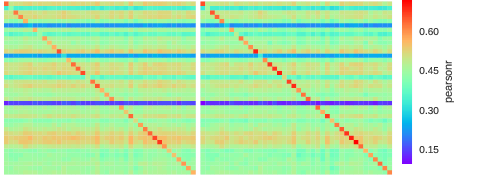
\includegraphics[width=1\linewidth]{figures/confusion_STORY-MATH.png}
  \caption{\textbf{Confusion matrices} for predicted versus true activation maps for
    the ``Story vs Math'' task contrast. The left plot corresponds to the reference
    method~\citep{tavor2016task} while the right one is for our proposed method.
      Higher diagonal values is better.
      The strong diagonal dorminance of these matrices reveals that the predicted maps of the subjects are more similar to their true maps than to other subjects.
      }
\label{fig:confusion}
\end{figure}

\begin{pagefigure}%[!htbp]
  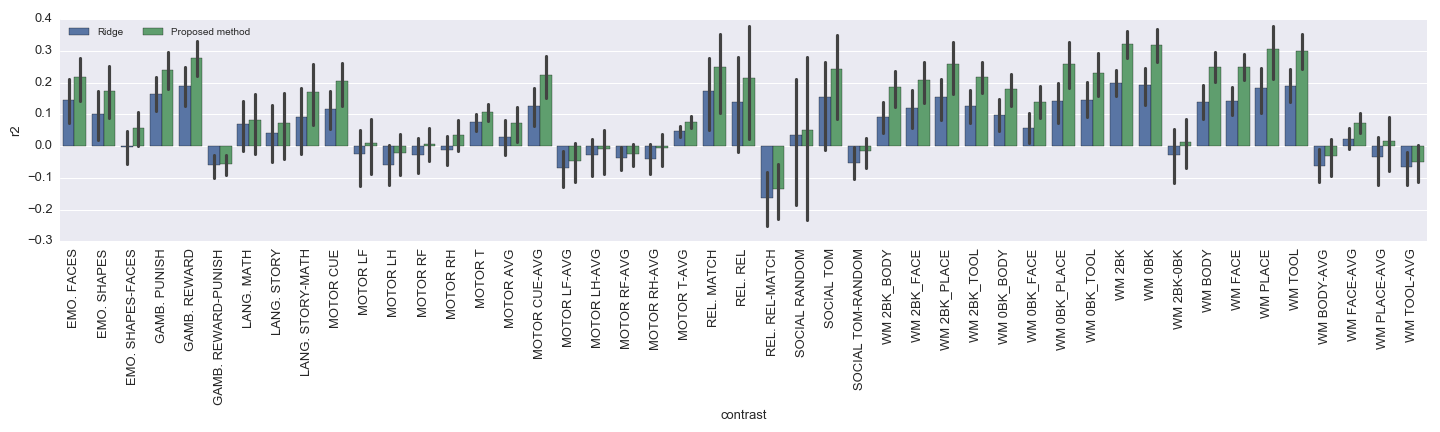
\includegraphics[width=1\linewidth]{figures/all_r2.png}
  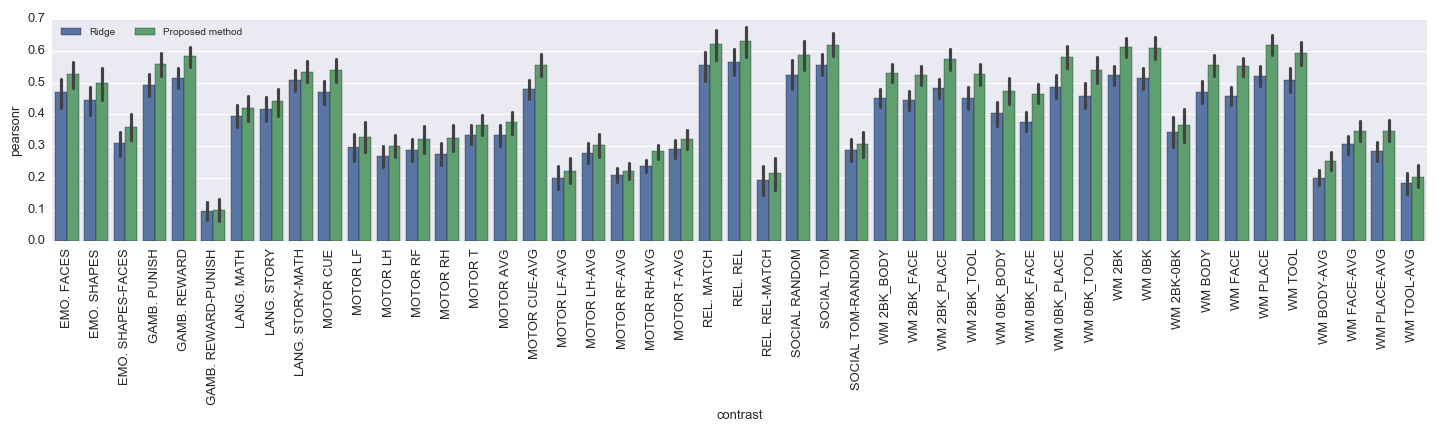
\includegraphics[width=1\linewidth]{figures/all_pearsonr.png}
  \caption{\textbf{Top:} $R^2$-score for predicting subject-specific activation maps for different task contrasts, from their resting data. These results are for the different contrasts of the HCP dataset~\citep{VanEssen20122222} are shown.
    Results for the reference method \citep{tavor2016task} are also shown.
    \textbf{Bottom:} Pearson correlation for the same prediction problem.
  }
  \label{fig:confusion_boxplots}
\end{pagefigure}

% \begin{pagefigure}%[!htbp]
%   \includegraphics[width=1\linewidth]{figures/{LANG._STORY-MATH_r2}.png}
%   \includegraphics[width=1\linewidth]{figures/{WM_2BK_r2}.png}
%   \includegraphics[width=1\linewidth]{figures/{WM_BODY-AVG_r2}.png}
%   \caption{...
%   }
%   \label{fig:subj_boxplots}
% \end{pagefigure}
  
% \begin{pagefigure}
% \subfloat[Shapes vs Faces] { 
%   \includegraphics[width=.33\linewidth]{figures/cmatrices/SHAPES-FACES.png}
% }
% \subfloat[Faces] {
%   \hspace{-.5em}
%   \includegraphics[width=.33\linewidth]{figures/cmatrices/FACES.png}
%   }
%   \hspace{-.5em}
% \subfloat[Shapes] {  
%   \includegraphics[width=.33\linewidth]{figures/cmatrices/SHAPES.png}
% }
% \hspace{-.5em}

% \subfloat[Reward vs Punish] { 
%   \includegraphics[width=.33\linewidth]{figures/cmatrices/REWARD-PUNISH.png}
% }
% \subfloat[Reward] {
%   \hspace{-.5em}
%   \includegraphics[width=.33\linewidth]{figures/cmatrices/REWARD.png}
%   }
%   \hspace{-.5em}
% \subfloat[Punish] {  
%   \includegraphics[width=.33\linewidth]{figures/cmatrices/PUNISH.png}
% }
% \hspace{-.5em}

% \subfloat[Story vs Math] { 
%   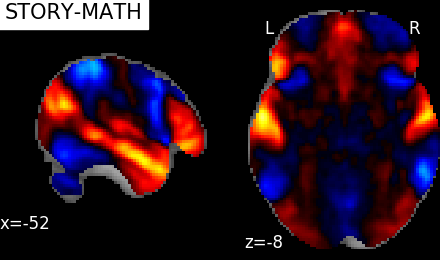
\includegraphics[width=.33\linewidth]{figures/cmatrices/STORY-MATH.png}
% }
% \subfloat[Story] {
%   \hspace{-.5em}
%   \includegraphics[width=.33\linewidth]{figures/cmatrices/STORY.png}
%   }
%   \hspace{-.5em}
% \subfloat[Math] {  
%   \includegraphics[width=.33\linewidth]{figures/cmatrices/MATH.png}
% }

% \hspace{-.5em}

% \subfloat[Tongue vs Avg] { 
%   \includegraphics[width=.33\linewidth]{figures/cmatrices/T-AVG.png}
% }
% \subfloat[Tongue] {
%   \hspace{-.5em}
%   \includegraphics[width=.33\linewidth]{figures/cmatrices/T.png}
%   }
%   \hspace{-.5em}
% \subfloat[Avg] {  
%   \includegraphics[width=.33\linewidth]{figures/cmatrices/AVG.png}
% }
% \hspace{-.5em}

% \subfloat[Rel vs Match] { 
%   \includegraphics[width=.33\linewidth]{figures/cmatrices/REL-MATCH.png}
% }
% \subfloat[Rel] {
%   \hspace{-.5em}
%   \includegraphics[width=.33\linewidth]{figures/cmatrices/REL.png}
%   }
%   \hspace{-.5em}
% \subfloat[Match] {  
%   \includegraphics[width=.33\linewidth]{figures/cmatrices/MATCH.png}
% }
% \hspace{-.5em}

% \subfloat[2BK vs 0BK] { 
%   \includegraphics[width=.33\linewidth]{figures/cmatrices/2BK-0BK.png}
% }
% \subfloat[2BK] {
%   \hspace{-.5em}
%   \includegraphics[width=.33\linewidth]{figures/cmatrices/2BK.png}
%   }
%   \hspace{-.5em}
% \subfloat[0BK] {  
%   \includegraphics[width=.33\linewidth]{figures/cmatrices/0BK.png}
% }
% \hspace{-.5em}

% \caption{\textbf{Confusion matrices} for the Pearson correlation between true and predicted $Z$-maps, for different task contrasts. \textbf{XXX: these figures should be regenerated with a pair of (vmin,vmax) per contrast!}}
% \end{pagefigure}

\paragraph{Qualitative metrics.} In Fig. \ref{fig:zmaps}, we display level-curves of the population mean (magenta) of
activation maps for the ``Story-vs-Math'' and ``2BK-vs-0BK'' task contrasts, superimposed on the true activation maps of the
subjects (the background image).  The population mean activation map (magenta) is shown as a baseline (dummy predictor).
We see that the contours for the predicted activation maps using our proposed method (green)
faithfully follow topography of the true activation maps, indicating that the model successfully
predicted the topography of the subjects' activation patterns for the contrasts.


\begin{pagefigure}
  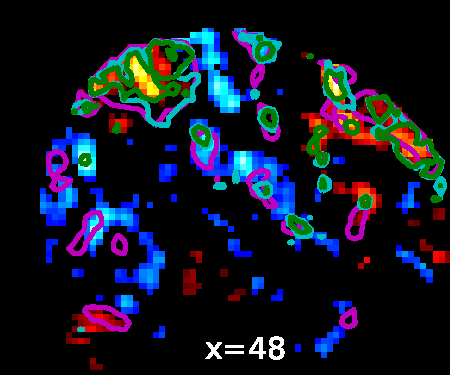
\includegraphics[width=.33\linewidth]{figures/brain_2BK-0BK_135528_01bags.pdf}
  \hspace{-.2cm}
  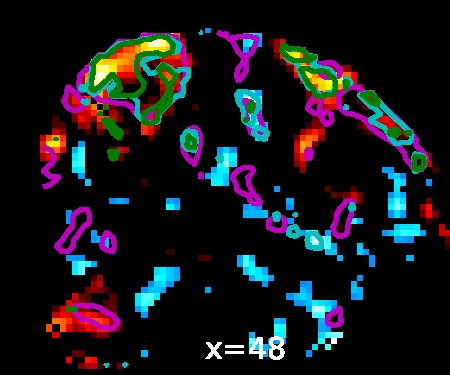
\includegraphics[width=.33\linewidth]{figures/brain_2BK-0BK_173536_01bags.pdf}
  \hspace{-.2cm}
  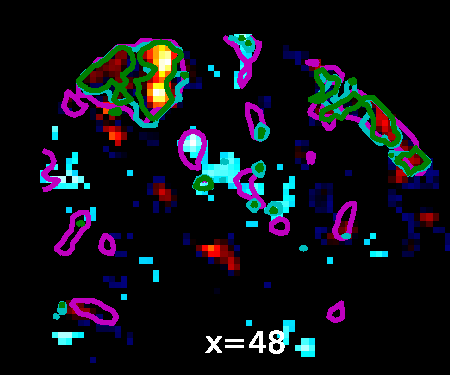
\includegraphics[width=.33\linewidth]{figures/brain_2BK-0BK_137633_01bags.pdf}
  \\
  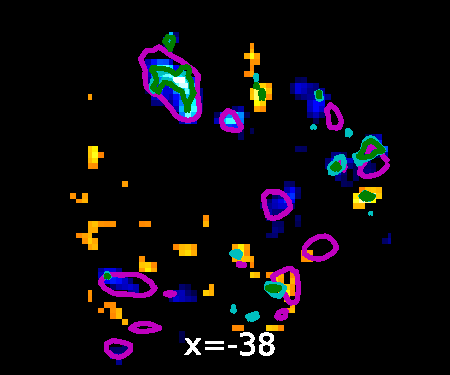
\includegraphics[width=.33\linewidth]{figures/brain_STORY-MATH_135528_01bags.pdf}
  \hspace{-.2cm}
  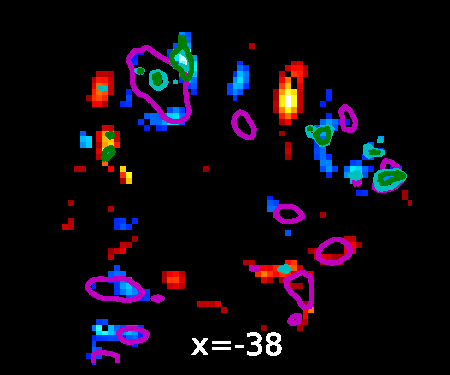
\includegraphics[width=.33\linewidth]{figures/brain_STORY-MATH_173536_01bags.pdf}
  \hspace{-.2cm}
  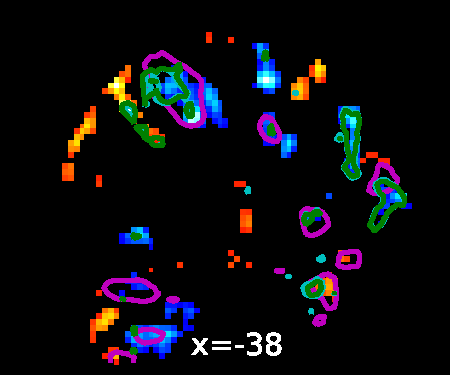
\includegraphics[width=.33\linewidth]{figures/brain_STORY-MATH_137633_01bags.pdf}
  \caption{Level-curves of the population mean (magenta), predicted activation
    maps using our proposed method (green) and the reference method \citep{tavor2016task}
    (cyan) for different contrasts. Each column represents a different subject (here 3),
    while each row represents a task contrast (here 2): first row is for ``2BK-0BK'' and second row is ``Story-vs-Math''.}
  \label{fig:zmaps}
\end{pagefigure}
  
\section{Concluding remarks}
We have proposed a general framework for the problem of predicting task fMRI activation maps
from resting-state-only features. Our method creates an ensemble of parcel-wise low-rank multi-target
linear models models, over different random sub-populations of the training subjects to leverage
the full richness of the data and jointly predict activation maps to different cognitive hypotheses
(task contrasts). This is a major improvement over the state of the art \citep{tavor2016task},
as confirmed by extensive experiments on real data. 

A practical implication of our results is that, for population
studies, a large amount of information can be captured solely by a T1
image + resting-state fMRI: faster, cheaper scanning OR more control on data quality
(imputation, outlier control). This explores new avenues for exploring
the human brain via resting-state data, in patients and healthy subjects alike.
\paragraph{Software} The code will be made publicly available online soon.

% \begin{proof}[Derivation of formula \eqref{eq:mr}]
%   \begin{eqnarray*}
%   \begin{split}
%     \tilde{\B{X}}_s(\lambda) &= (\A_s^T\A_ss + \lambda \Id_k)^{-1}\A_s^T\B{X}_s \\
%     &= ((\B{D}\B{D}^T)^{-1}\B{D}\B{X}_s^T\B{X}_s\B{D}^T(\B{D}\B{D}^T)^{-1}  + \lambda \Id_k)^{-1}(\B{D}\B{D}^T)^{-1}\B{D}\B{X}_s^T\B{X}_s\\
%     &= \B{D}\B{D}^T\underbrace{(\B{D}\B{X}_s^T\B{X}_s\B{D}^T  + \lambda \Id_k)^{-1}\B{D}\B{X}_s^T\B{X}_s}_{\text{Ridge}_\lambda(\B{X}_s\B{D}^T,\B{X}_s)}
%      = \B{D}\B{D}^T\B{D}\B{X}_s^T(\B{X}_s\B{D}^T\B{D}\B{X}_s^T  + \lambda \Id_n)^{-1}\B{X}_s.
%   \end{split}
% \end{eqnarray*}
% In the limit $\lambda \rightarrow 0^+$, we get \eqref{eq:mr}.
% \qed
% \end{proof}

% \clearpage
\bibliographystyle{plainnat}
\bibliography{bib_all}
